\section*{Aufgabe 10 - Eingeschränkte Kanäle}
\addcontentsline{toc}{subsection}{Aufgabe 10 - Eingeschränkte Kanäle}
\begin{paragraph}{1)}
  \[ L = (0 | 10)^* (1 | \epsilon) \]
  \[ K = (0 | 1 | \epsilon) (0 (0^+) | 1 (1^+))^* (0 | 1 | \epsilon) \]
  \[ M = (\epsilon | 1 | 11) ((0 | 00) (1 | 11))^* (\epsilon | 0 | 00) \]
\end{paragraph}
\begin{paragraph}{2)}
  Die umrahmten Bereiche enthalten die Zustände, die für
  das asymptotische Wachstum relevant sind.

  \begin{tikzpicture}[shorten >=1pt,node distance=2cm,on grid,auto]
    % helper grid
    % \draw[help lines] (-1,-10) grid (10,2);
    % L
    \draw[fill=orange!25,rounded corners=5pt] (-0.8,-2.7) rectangle (0.8,1.5);
    \node[state,initial,initial text=L,accepting] (A)                 {$A$};
    \node[state,accepting]                (B)    [below=of A]         {$B$};
    \node[state]                          (C)    [above right=of B]   {$C$};
    \path[->] (A) edge [loop above] node        {0} ()
                  edge [bend left]  node        {1} (B)
              (B) edge [bend left]  node        {0} (A)
                  edge              node [swap] {1} (C)
              (C) edge [loop right] node        {0,1} ();
    % K
    \draw[fill=red!25,rounded corners=5pt] (4.7,-4.9) rectangle (8.1,1.0);
    \node[state,initial,initial text=K,accepting] (FK)   at (4,-2)    {$F$};
    \node[state,accepting]                (AK)   [above right=of FK]  {$A$};
    \node[state,accepting]                (CK)   [below right=of FK]  {$C$};
    \node[state,accepting]                (BK)   [right=of AK]        {$B$};
    \node[state,accepting]                (DK)   [right=of CK]        {$D$};
    \node[state]                          (EK)   [above right=of DK]  {$E$};
    \path[->] (FK) edge              node            {0} (AK)
                   edge              node [swap]     {1} (CK)
              (AK) edge [loop above] node            {0} ()
                   edge              node            {1} (BK)
              (BK) edge              node            {0} (EK)
                   edge              node [near end] {1} (CK)
              (CK) edge              node [swap]     {0} (DK)
                   edge [loop below] node            {1} ()
              (DK) edge              node [near end] {0} (AK)
                   edge              node [swap]     {1} (EK)
              (EK) edge [loop right] node            {0,1} ();
    % M
    \draw[fill=purple!25,rounded corners=5pt] (-0.3,-8) rectangle (3.1,-4);
    \node[state,initial,initial text=M,accepting] (AM) at (-1,-6)      {$A$};
    \node[state,accepting]                (BM) [above right=of AM]     {$B$};
    \node[state,accepting]                (CM) [right=of BM]           {$C$};
    \node[state,accepting]                (DM) [below right=of AM]     {$D$};
    \node[state,accepting]                (EM) [right=of DM]           {$E$};
    \node[state]                          (FM) [above right=of EM]     {$F$};
    \path[->] (AM) edge              node                   {0} (BM)
                   edge              node [swap]            {1} (DM)
              (BM) edge              node                   {0} (CM)
                   edge              node                   {1} (DM)
              (CM) edge              node                   {0} (FM)
                   edge              node [near start,swap] {1} (DM)
              (DM) edge [bend left]  node [swap]            {0} (BM)
                   edge              node                   {1} (EM)
              (EM) edge              node [near start,swap] {0} (BM)
                   edge              node [swap]            {1} (FM)
              (FM) edge [loop right] node                   {0,1} ();
  \end{tikzpicture}
\end{paragraph}
\begin{paragraph}{3)} Trellis-Diagramme:
\begin{itemize}
  \item $L$:

    \newcounter{x}
    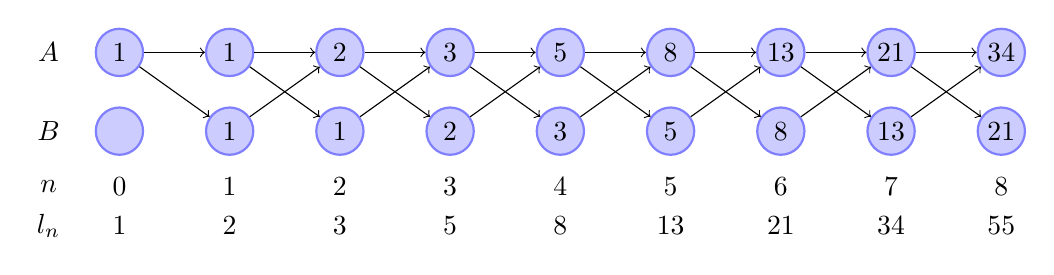
\begin{tikzpicture}[place/.style={circle,draw=blue!50,fill=blue!20,thick,
                        inner sep=0pt,minimum size=6mm}]
      \node at (0.5,0) {$A$};
      \foreach \x/\xtext in {1/1,2/1,3/2,4/3,5/5,6/8,7/13,8/21,9/34}
        \node[xshift=\x*1.4 cm] (T-0-\x) [place] at (0,0) {$\xtext$};
      \node at (0.5,-1) {$B$};
      \foreach \x/\xtext in {1/,2/1,3/1,4/2,5/3,6/5,7/8,8/13,9/21}
        \node[xshift=\x*1.4 cm] (T-1-\x) [place] at (0,-1) {$\xtext$};
      \foreach \x in {1,...,8}
        \setcounter{x}{\x}\stepcounter{x}
        \path[->] (T-0-\x) edge (T-0-\arabic{x})
                           edge (T-1-\arabic{x});
      \foreach \x in {2,...,8}
        \setcounter{x}{\x}\stepcounter{x}
        \path[->] (T-1-\x) edge (T-0-\arabic{x});
      \node at (0.5,-1.7) {$n$};
      \node at (0.5,-2.2) {$l_n$};
      \foreach \x/\y in {0/1,1/2,2/3,3/5,4/8,5/13,6/21,7/34,8/55} {
        \node[xshift=\x*1.4 cm] at (1.4,-1.7) {$\x$};
        \node[xshift=\x*1.4 cm] at (1.4,-2.2) {$\y$};
      }
    \end{tikzpicture}
    \[ (l_n)_{0\leq n\leq8} = (1, 2, 3, 5, 8, 13, 21, 34, 55) \]
  \item $K$:

    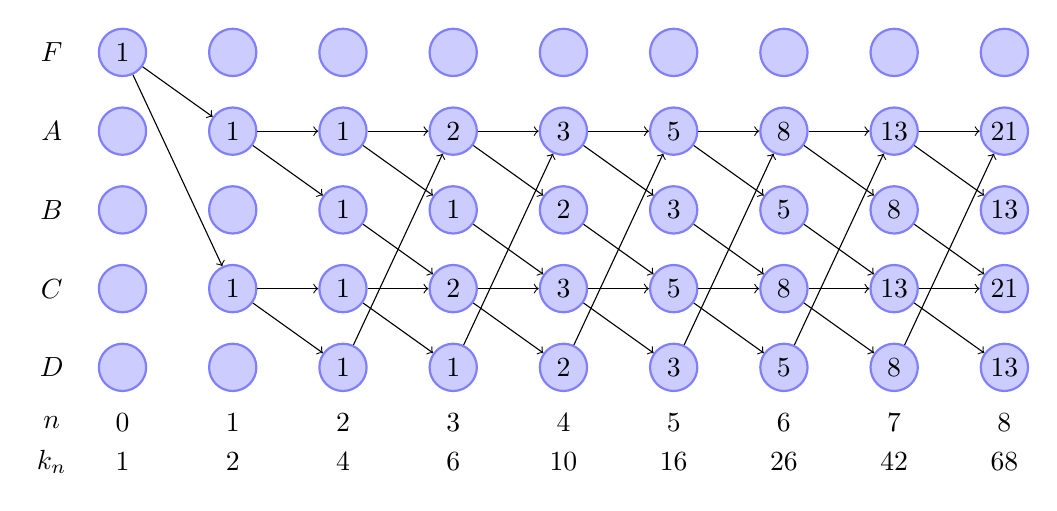
\begin{tikzpicture}[place/.style={circle,draw=blue!50,fill=blue!20,thick,
                        inner sep=0pt,minimum size=6mm}]
      \node at (0.5,0) {$F$};
      \foreach \x/\xtext in {1/1,2/,3/,4/,5/,6/,7/,8/,9/}
        \node[xshift=\x*1.4 cm] (T-0-\x) [place] at (0,0) {$\xtext$};
      \node at (0.5,-1) {$A$};
      \foreach \x/\xtext in {1/,2/1,3/1,4/2,5/3,6/5,7/8,8/13,9/21}
        \node[xshift=\x*1.4 cm] (T-1-\x) [place] at (0,-1) {$\xtext$};
      \node at (0.5,-2) {$B$};
      \foreach \x/\xtext in {1/,2/,3/1,4/1,5/2,6/3,7/5,8/8,9/13}
        \node[xshift=\x*1.4 cm] (T-2-\x) [place] at (0,-2) {$\xtext$};
      \node at (0.5,-3) {$C$};
      \foreach \x/\xtext in {1/,2/1,3/1,4/2,5/3,6/5,7/8,8/13,9/21}
        \node[xshift=\x*1.4 cm] (T-3-\x) [place] at (0,-3) {$\xtext$};
      \node at (0.5,-4) {$D$};
      \foreach \x/\xtext in {1/,2/,3/1,4/1,5/2,6/3,7/5,8/8,9/13}
        \node[xshift=\x*1.4 cm] (T-4-\x) [place] at (0,-4) {$\xtext$};
      % connections
      \path[->] (T-0-1) edge (T-1-2) edge (T-3-2);
      \foreach \x in {2,...,8} {
        \setcounter{x}{\x}\stepcounter{x}
        \path[->] (T-1-\x) edge (T-1-\arabic{x})
                           edge (T-2-\arabic{x});
        \path[->] (T-3-\x) edge (T-3-\arabic{x})
                           edge (T-4-\arabic{x});
      }
      \foreach \x in {3,...,8} {
        \setcounter{x}{\x}\stepcounter{x}
        \path[->] (T-2-\x) edge (T-3-\arabic{x});
        \path[->] (T-4-\x) edge (T-1-\arabic{x});
      }
      \node at (0.5,-4.7) {$n$};
      \node at (0.5,-5.2) {$k_n$};
      \foreach \x/\y in {0/1,1/2,2/4,3/6,4/10,5/16,6/26,7/42,8/68} {
        \node[xshift=\x*1.4 cm] at (1.4,-4.7) {$\x$};
        \node[xshift=\x*1.4 cm] at (1.4,-5.2) {$\y$};
      }
    \end{tikzpicture}
    \[ (k_n)_{0\leq n\leq8} = (1, 2, 4, 6, 10, 16, 26, 42, 68) \]
  \item $M$:

    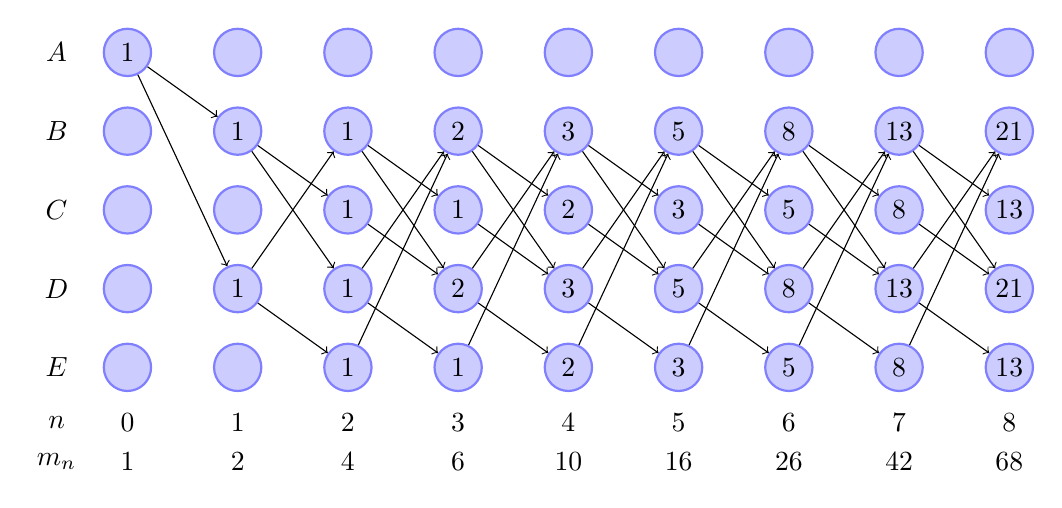
\begin{tikzpicture}[place/.style={circle,draw=blue!50,fill=blue!20,thick,
                        inner sep=0pt,minimum size=6mm}]
      \node at (0.5,0) {$A$};
      \foreach \x/\xtext in {1/1,2/,3/,4/,5/,6/,7/,8/,9/}
        \node[xshift=\x*1.4 cm] (T-0-\x) [place] at (0,0) {$\xtext$};
      \node at (0.5,-1) {$B$};
      \foreach \x/\xtext in {1/,2/1,3/1,4/2,5/3,6/5,7/8,8/13,9/21}
        \node[xshift=\x*1.4 cm] (T-1-\x) [place] at (0,-1) {$\xtext$};
      \node at (0.5,-2) {$C$};
      \foreach \x/\xtext in {1/,2/,3/1,4/1,5/2,6/3,7/5,8/8,9/13}
        \node[xshift=\x*1.4 cm] (T-2-\x) [place] at (0,-2) {$\xtext$};
      \node at (0.5,-3) {$D$};
      \foreach \x/\xtext in {1/,2/1,3/1,4/2,5/3,6/5,7/8,8/13,9/21}
        \node[xshift=\x*1.4 cm] (T-3-\x) [place] at (0,-3) {$\xtext$};
      \node at (0.5,-4) {$E$};
      \foreach \x/\xtext in {1/,2/,3/1,4/1,5/2,6/3,7/5,8/8,9/13}
        \node[xshift=\x*1.4 cm] (T-4-\x) [place] at (0,-4) {$\xtext$};
      % connections
      \path[->] (T-0-1) edge (T-1-2) edge (T-3-2);
      \foreach \x in {2,...,8} {
        \setcounter{x}{\x}\stepcounter{x}
        \path[->] (T-1-\x) edge (T-2-\arabic{x})
                           edge (T-3-\arabic{x});
        \path[->] (T-3-\x) edge (T-1-\arabic{x})
                           edge (T-4-\arabic{x});
      }
      \foreach \x in {3,...,8} {
        \setcounter{x}{\x}\stepcounter{x}
        \path[->] (T-2-\x) edge (T-3-\arabic{x});
        \path[->] (T-4-\x) edge (T-1-\arabic{x});
      }
      \node at (0.5,-4.7) {$n$};
      \node at (0.5,-5.2) {$m_n$};
      \foreach \x/\y in {0/1,1/2,2/4,3/6,4/10,5/16,6/26,7/42,8/68} {
        \node[xshift=\x*1.4 cm] at (1.4,-4.7) {$\x$};
        \node[xshift=\x*1.4 cm] at (1.4,-5.2) {$\y$};
      }
    \end{tikzpicture}
    \[ (m_n)_{0\leq n\leq8} = (1, 2, 4, 6, 10, 16, 26, 42, 68) \]
\end{itemize}
\end{paragraph}
\begin{paragraph}{4)}
  Die Folgen $(l_n), (k_n)$ und $(m_n)$ wachsen wie die Fibonacci-Zahlen.
  $(l_n)$ ist sogar genau die Fibonacci-Folge.
\end{paragraph}
\begin{paragraph}{5)}
  \[ L = \begin{bmatrix} 1 & 1 \\ 1 & 0 \end{bmatrix} \]
  \[ \chi_L(\lambda) = det(L - \lambda \cdot \mathds{1}) 
     = (1 - \lambda)(-\lambda) - 1 = \lambda^2 - \lambda - 1 \]
  Eigenwerte:
  \[ \chi_L(\lambda) = 0 \Rightarrow \lambda_1 
     = \Phi, \quad \lambda_2 = \hat \Phi \] \\[2em]
  \[ K = \begin{bmatrix} 1 & 1 & 0 & 0 \\ 0 & 0 & 1 & 0 \\
                         0 & 0 & 1 & 1 \\ 1 & 0 & 0 & 0 \end{bmatrix} \]
  \[ \chi_K(\lambda) = det(K - \lambda \cdot \mathds{1})
     = \begin{vmatrix} 1-\lambda & 1 & 0 & 0 \\
                       0 & -\lambda & 1 & 0 \\
                       0 & 0 & 1-\lambda & 1 \\
                       1 & 0 & 0 & -\lambda \end{vmatrix} = \]
  \[ = -\lambda \cdot \begin{vmatrix} 1-\lambda & 0 & 0 \\ 
                                      0 & 1-\lambda & 1 \\
                                      1 & 0 & -\lambda \end{vmatrix} -
                      \begin{vmatrix} 1-\lambda & 1 & 0 \\
                                      0 & 0 & 1 \\
                                      1 & 0 & -\lambda \end{vmatrix} = \]
  \[ = (-\lambda)^2 (1-\lambda)^2 - 1 = \]
  \[ = \lambda^2 (1 - 2\lambda + \lambda^2) - 1 = \]
  \[ = \lambda^4 - 2\lambda^3 +\lambda^2 - 1 \]
  Eigenwerte:
  \[ \chi_K(\lambda) = 0 \Leftrightarrow (\lambda^2 - \lambda)^2 - 1 
     = 0 \Leftrightarrow \lambda^2 - \lambda \pm 1 = 0 \]
  \[ \lambda_1 = \frac{1 + i\sqrt{3}}{2}, \quad
     \lambda_2 = \frac{1 - i\sqrt{3}}{2} \]
  \[ \lambda_3 = \Phi, \quad \lambda_4 = \hat \Phi \] \\[2em]
  \[ M = \begin{bmatrix} 0 & 1 & 1 & 0 \\ 0 & 0 & 1 & 0 \\
                         1 & 0 & 0 & 1 \\ 1 & 0 & 0 & 0 \end{bmatrix} \]
  \[ \chi_M(\lambda) = det(M - \lambda \cdot \mathds{1})
     = \begin{vmatrix} -\lambda & 1 & 1 & 0 \\
                       0 & -\lambda & 1 & 0 \\
                       1 & 0 & -\lambda & 1 \\
                       1 & 0 & 0 & -\lambda \end{vmatrix} = \]
  \[ = -\begin{vmatrix} 1 & 1 & 0 \\ 
                        -\lambda & 1 & 0 \\
                        0 & -\lambda & 1 \end{vmatrix} - \lambda \cdot
        \begin{vmatrix} -\lambda & 1 & 1 \\
                        0 & -\lambda & 1 \\
                        1 & 0 & -\lambda \end{vmatrix} = \]
  \[ = -(1 + \lambda) - \lambda ((-\lambda)^3 + 1 - (-\lambda)) = \]
  \[ = - 1 - \lambda - \lambda ((-\lambda)^3 + 1 + \lambda) = \]
  \[ = \lambda^4 - \lambda^2 - 2\lambda - 1 \]
  Eigenwerte:
  \[ \chi_M(\lambda) = 0 \Leftrightarrow 
     ((\lambda + 1) - \lambda^2)((\lambda + 1) + \lambda^2) = 0
     \Leftrightarrow \pm \lambda^2 + \lambda + 1 = 0 \]
  \[ \lambda_1 = \frac{-1 + i\sqrt{3}}{2}, \quad
     \lambda_2 = \frac{-1 - i\sqrt{3}}{2} \]
  \[ \lambda_3 = \Phi, \quad \lambda_4 = \hat \Phi \]
  Der dem Betrag nach größte Eigenwert ist jeweils der goldene Schnitt $\Phi =
  \frac{1 + \sqrt{5}}{2}$.
\end{paragraph}
